\documentclass{beamer}
\usetheme{Berlin}

\title{Systems with a Small Number of
Variables}
\subtitle{Course: Complex Systems Modeling}
\author{Robert Flassig}
\institute{Brandenburg University of Applied Sciences}
\date{\today}

\begin{document}
\begin{frame}
\titlepage
\end{frame}

\begin{frame}
\frametitle{Outline}
\tableofcontents
\end{frame}

\section{Basics of Dynamical Systems}

\begin{frame}
    \frametitle{What Are Dynamical Systems?}
    {\small

    \textbf{Dynamical systems theory} is the foundation of rule-based models for complex systems. It focuses on \textbf{how systems change over time}, rather than on static properties.

    \bigskip

     \begin{block}{Definition}
     A dynamical system is a system whose state is uniquely specified by a set of variables and whose behavior is governed by predefined rules.
 \end{block}
    \bigskip

    \textbf{Examples of Dynamical Systems:}
    \begin{itemize}
        \item Population growth
        \item Swinging pendulum
        \item Celestial motions
        \item Behavior of rational individuals in negotiation games
    \end{itemize}

    \bigskip
}
\end{frame}
\begin{frame}
    \frametitle{What Are Dynamical Systems?}
   \textbf{Note:} A traditional definition of dynamical systems considers deterministic systems only, but stochastic (i.e.,
	probabilistic) behaviors can also be modeled in a dynamical system by, for example, representing the probability distribution of the system's states as a meta-level state.

  \bigskip

    \textbf{Question:} Can human behavior be modeled as a deterministic dynamical system?
    \begin{itemize}
        \item If individuals make decisions rationally, interactions may be modeled as deterministic.
        \item However, the validity of such a model depends on critical evaluation of underlying assumptions.
    \end{itemize}
   
\end{frame}


\begin{frame}
    \frametitle{Discrete-Time Dynamical System}

    A discrete-time dynamical system is represented by the equation:
    \[
    x_t = F(x_{t-1}, t)
    \]
    where \( x_t \) is the state of the system at time \( t \), and \( F \) is a function describing the system's evolution.

    \begin{itemize}
        \item Known as a \textbf{difference equation}, \textbf{recurrence equation}, or \textbf{iterative map} (when independent of \( t \)).
    \end{itemize}

\end{frame}

\begin{frame}
    \frametitle{Continuous-Time Dynamical System}

    A continuous-time dynamical system is defined by:
    \[
    \frac{dx}{dt} = F(x, t)
    \]
    where \( \frac{dx}{dt} \) describes the rate of change of the state variable \( x \) over time.

    \begin{itemize}
        \item Known as a \textbf{differential equation}.
    \end{itemize}

\end{frame}


\begin{frame}
    \frametitle{State Variables and Function \( F \)}

    \begin{itemize}
        \item In both discrete and continuous systems, \( x_t \) (or \( x \)) represents the \textbf{state variable} at time \( t \).
        \item The function \( F \) determines the rules by which the system evolves over time.
    \end{itemize}

    \bigskip

    The examples we are looking at are \textbf{first-order} dynamical systems (only dependent on the previous time step or first derivative), which can model a broad range of dynamics.
\end{frame}

\section{Examples}

\begin{frame}
    \frametitle{Example 1: Linear Difference Equation}

    The simplest discrete-time dynamical system:
    \[
    x_t = a x_{t-1} + b
    \]
    \begin{itemize}
        \item \(a\): growth or decay rate
        \item \(b\): constant input or forcing term
        \item \textbf{Fixed point:} \(x^* = \frac{b}{1-a}\), provided \(a \neq 1\)
        \item If \(|a| < 1\), the system converges to \(x^*\) (stable attractor)
    \end{itemize}

    \vspace{0.5em}
    \textit{Example:} Bank account balance with interest \(a\) and regular deposit \(b\).
\end{frame}

\begin{frame}
    \frametitle{Example 2: Nonlinear Iterative Map — Logistic Equation}

    The logistic map models population growth with limited resources:
    \[
    x_{t+1} = r\,x_t(1 - x_t)
    \]
    \begin{itemize}
        \item \(r\): growth rate parameter
        \item For small \(r\): converges to a fixed point
        \item For larger \(r\): exhibits oscillations and chaos
        \item Demonstrates how simple nonlinear rules can yield complex dynamics
    \end{itemize}

    \vspace{0.5em}
    \textit{Typical behavior:} bifurcations, period-doubling, and chaotic attractors.
\end{frame}

\begin{frame}
    \frametitle{Example 3: Physical Analogy — Damped Pendulum}

    Consider a pendulum in a dissipative (frictional) environment:
    \[
    \theta_{t+1} = \theta_t + \dot{\theta}_t, \quad
    \dot{\theta}_{t+1} = \dot{\theta}_t - \gamma \dot{\theta}_t - \sin(\theta_t)
    \]
    \begin{itemize}
        \item \(\gamma\): damping coefficient
        \item Without damping (\(\gamma = 0\)): perpetual oscillation — no attractor
        \item With damping: energy dissipates $\Rightarrow$ pendulum settles at bottom
        \item Bottom position = \textbf{stable fixed-point attractor}
    \end{itemize}

    \vspace{0.5em}
    \textit{Analogy:} Dissipation leads to convergence toward an attractor.
\end{frame}

\begin{frame}
    \frametitle{Example 4: Engineering System — Temperature Control}
{\small
    In engineering, many systems can be modeled by discrete-time updates of a physical variable.
    \[
    T_{t+1} = T_t + \Delta t \cdot k \, (T_{\text{set}} - T_t)
    \]
    \begin{itemize}
        \item \(T_t\): current temperature
        \item \(T_{\text{set}}\): desired (setpoint) temperature
        \item \(k\): control gain (heat transfer or proportional control constant)
        \item \(\Delta t\): time step
    \end{itemize}

    \vspace{0.5em}
    \textbf{Interpretation:}
    \begin{itemize}
        \item The system updates its state proportionally to the temperature error.
        \item If \(0 < \Delta t \, k < 1\), the system converges smoothly to the setpoint.
        \item The steady-state value \(T^* = T_{\text{set}}\) is a \textbf{stable attractor}.
    \end{itemize}

    \vspace{0.5em}
    \textit{Example:} Electric heater with proportional control or cooling of a heated metal part.
    }
\end{frame}


\begin{frame}
    \frametitle{Example 5: Mechanical Engineering System — Mass–Spring–Damper}

    A classic example of a dynamical system is the mass–spring–damper:
    \[
    m \ddot{x} + c \dot{x} + k x = F(t)
    \]

    Discretizing in time (e.g., with time step $\Delta t$):
    \[
    x_{t+1} = x_t + \Delta t \, \dot{x}_t
    \]
    \[
    \dot{x}_{t+1} = \dot{x}_t + \frac{\Delta t}{m} \big(F_t - c \dot{x}_t - k x_t \big)
    \]

    \begin{itemize}
        \item \(m\): mass, \(c\): damping coefficient, \(k\): stiffness
        \item If \(F_t = 0\), the system oscillates and gradually settles due to damping
        \item Equilibrium \(x^* = 0, \dot{x}^* = 0\) is a \textbf{stable fixed-point attractor}
    \end{itemize}

    \vspace{0.5em}
    \textit{Example:} Vehicle suspension, vibration absorber, or robotic actuator.
\end{frame}



\begin{frame}
    \frametitle{Modeling Goal \& Setup: Wind Turbine Tower in Tower-Shadow Excitation}

    \textbf{Objective:} Model lateral vibration of the tower (top deflection $x(t)$) excited by periodic aerodynamic loads when blades pass the tower's wind shadow.

    \textbf{System boundary:} Tower as a single bending mode (lumped at nacelle/top).

    \textbf{Assumptions (idealizations):}
    \begin{itemize}
        \item Single DoF (first lateral bending mode dominates)
        \item Linear behavior near operating point
        \item Small vibrations, constant properties
        \item Harmonic external force from blade passing
    \end{itemize}

    \textbf{Inputs/Outputs:}
    \begin{itemize}
        \item Input: harmonic force $F(t) = F_0 \sin(\Omega t)$
        \item Output: lateral displacement $x(t)$ at tower top
    \end{itemize}
\end{frame}

\begin{frame}
    \frametitle{From Physics to Differential Equation}

    \textbf{Model choice:} Mass–spring–damper for the first mode
    \[
    m \ddot{x}(t) + c \dot{x}(t) + k x(t) = F_0 \sin(\Omega t)
    \]

    \textbf{Parameters:}
    \[
    \omega_n = \sqrt{\frac{k}{m}}, \qquad
    \zeta = \frac{c}{2\sqrt{km}}
    \]

    \textbf{State-space (if desired):}
    \[
    \dot{x}_1 = x_2, \qquad
    \dot{x}_2 = -2\zeta \omega_n x_2 - \omega_n^2 x_1 + \frac{F_0}{m}\sin(\Omega t)
    \]

    \textbf{Interpretation:}
    \begin{itemize}
        \item $m$: modal mass of first mode
        \item $k$: modal stiffness (from $\omega_n$)
        \item $c$: modal damping (from $\zeta$)
    \end{itemize}
\end{frame}

\begin{frame}
    \frametitle{Excitation Frequency from Blade Passing}

    \textbf{Blade-passing frequency (BPF):}
    \[
    \Omega = N_b \,\omega_r, \qquad
    \omega_r = \frac{2\pi\,n_{\mathrm{rpm}}}{60}
    \]
    where $N_b$ = number of blades,\; $n_{\mathrm{rpm}}$ = rotor speed.

    \textbf{Example:}
    \begin{itemize}
        \item $N_b = 3$, \quad $n_{\mathrm{rpm}} = 15$
        \item $\omega_r = 2\pi \cdot 15/60 = \frac{\pi}{2}\ \mathrm{rad/s}$
        \item $\Omega = 3 \cdot \frac{\pi}{2} = \frac{3\pi}{2} \approx 4.71\ \mathrm{rad/s}$
        \item $f_{\mathrm{BPF}} = \Omega/(2\pi) \approx 0.75\ \mathrm{Hz}$
    \end{itemize}

    \textbf{Note:} Yaw misalignment, shear, and tower–nacelle aerodynamics make $F_0$ and $\Omega$ slightly time-varying in reality — we use a constant-$\Omega$ sinusoid as a first model.
\end{frame}

\begin{frame}
    \frametitle{Steady-State Response \& Resonance Insight}
{\small
    \textbf{Harmonic steady-state amplitude} ($x(t)=X\sin(\Omega t - \phi)$):
    \[
    X(\Omega) = \frac{F_0/k}{\sqrt{\left(1 - \left(\frac{\Omega}{\omega_n}\right)^2\right)^2 + \left(2\zeta \frac{\Omega}{\omega_n}\right)^2}}
    \]
    \[
    \phi(\Omega) = \arctan\!\left(\frac{2\zeta \,\Omega/\omega_n}{\,1 - (\Omega/\omega_n)^2\,}\right)
    \]

    \textbf{Key engineering points:}
    \begin{itemize}
        \item \textbf{Resonance risk} when $\Omega \approx \omega_n$
        \item Higher damping ($\zeta$) lowers peak amplitude
        \item Detuning: design $\omega_n$ away from dominant excitations
    \end{itemize}

    \textbf{Quick check (numbers):}
    \begin{itemize}
        \item $\omega_n = 5.5\ \mathrm{rad/s}$,\; $\zeta = 0.02$,\; $\Omega = 4.71\ \mathrm{rad/s}$,\; $F_0/k = 0.02\ \mathrm{m}$
        \item $X \approx \frac{0.02}{\sqrt{(1-(4.71/5.5)^2)^2 + (2\cdot 0.02\cdot 4.71/5.5)^2}} \approx 0.036\ \mathrm{m}$
    \end{itemize}
}
\end{frame}

\begin{frame}
    \frametitle{Modeling Process Checklist \& Next Steps}

    \textbf{Modeling steps students should follow:}
    \begin{enumerate}
        \item \textbf{Define} the question and outputs ($x(t)$ at tower top)
        \item \textbf{Choose} an appropriate model (1-DoF MSD for first mode)
        \item \textbf{Idealize} (linearity, small motion, harmonic input)
        \item \textbf{Parameterize} ($\omega_n, \zeta$ from tests or design data)
        \item \textbf{Relate excitation} ($\Omega = N_b \omega_r$; estimate $F_0$)
        \item \textbf{Analyze} $X(\Omega)$ and \textbf{check resonance margins}
        \item \textbf{Decide} mitigations: detune $\omega_n$, increase damping, or avoid critical rotor speeds (operational window)
    \end{enumerate}

    \textbf{Extensions (optional):}
    \begin{itemize}
        \item Include higher modes (MDOF), stochastic wind loads, or operational speed ramps
        \item Compare analytical $X(\Omega)$ with time-domain simulation
    \end{itemize}
\end{frame}

\begin{frame}
    \frametitle{Reflection 1}

    \textbf{Question:} Have you learned of any models in the natural or social sciences that are formulated as either discrete-time or continuous-time dynamical systems?

    \begin{itemize}
        \item If so, what are they?
        \item What assumptions do these models rely on?
    \end{itemize}
\end{frame}

\begin{frame}
    \frametitle{Reflection 2}

    \textbf{Question:} What are some appropriate choices for state variables in the following systems?
    \begin{itemize}
        \item Population growth
        \item Swinging pendulum
        \item Motions of celestial bodies
        \item Behavior of \emph{rational individuals} in a negotiation game
    \end{itemize}

\end{frame}

\section{Phase Space}
% Slide 1: Introduction to Phase Space
\begin{frame}
    \frametitle{Phase Space}

    \textbf{Phase space} is a conceptual tool used to analyze the behavior of dynamical systems.

    \begin{itemize}
        \item It is a theoretical space where each state of the system is mapped to a unique spatial location.
        \item By studying the system in phase space, we gain insights into how the system evolves over time.
    \end{itemize}

\end{frame}

% Slide 2: Definition of Phase Space
\begin{frame}
    \frametitle{Definition of Phase Space}

    \begin{block}{Definition}
        A \textbf{phase space} of a dynamical system is a theoretical space where every state of the system corresponds to a unique location.
    \end{block}

    \bigskip

    \textbf{Degrees of freedom} represent the number of state variables needed to fully describe the system.
\end{frame}

% Slide 3: Degrees of Freedom and Dimensions of Phase Space
\begin{frame}
    \frametitle{Degrees of Freedom and Dimensions of Phase Space}

    \begin{itemize}
        \item Each degree of freedom in a system corresponds to an axis in its phase space.
        \item The dimensionality of phase space is equal to the number of degrees of freedom.
    \end{itemize}

    \bigskip

    For instance, a system with two degrees of freedom will have a 2-dimensional phase space.
\end{frame}

% Slide 4: Example: Ball Thrown Upward
\begin{frame}
    \frametitle{Example: Ball Thrown Upward 1/2}

    Consider a ball thrown upward in a frictionless vertical tube:

    \begin{itemize}
        \item This system has \textbf{two degrees of freedom}: position and velocity.
        \item We can represent the state of the ball in a 2-dimensional phase space with:
        \begin{itemize}
            \item Position on one axis
            \item Velocity on the other axis
        \end{itemize}
    \end{itemize}

    This phase space describes the system's behavior until the ball hits the bottom again.
\end{frame}

% Slide: Benefits of Drawing a Phase Space
\begin{frame}
    \frametitle{Example: Ball Thrown Upward 2/2}

    \begin{figure}
        \centering
        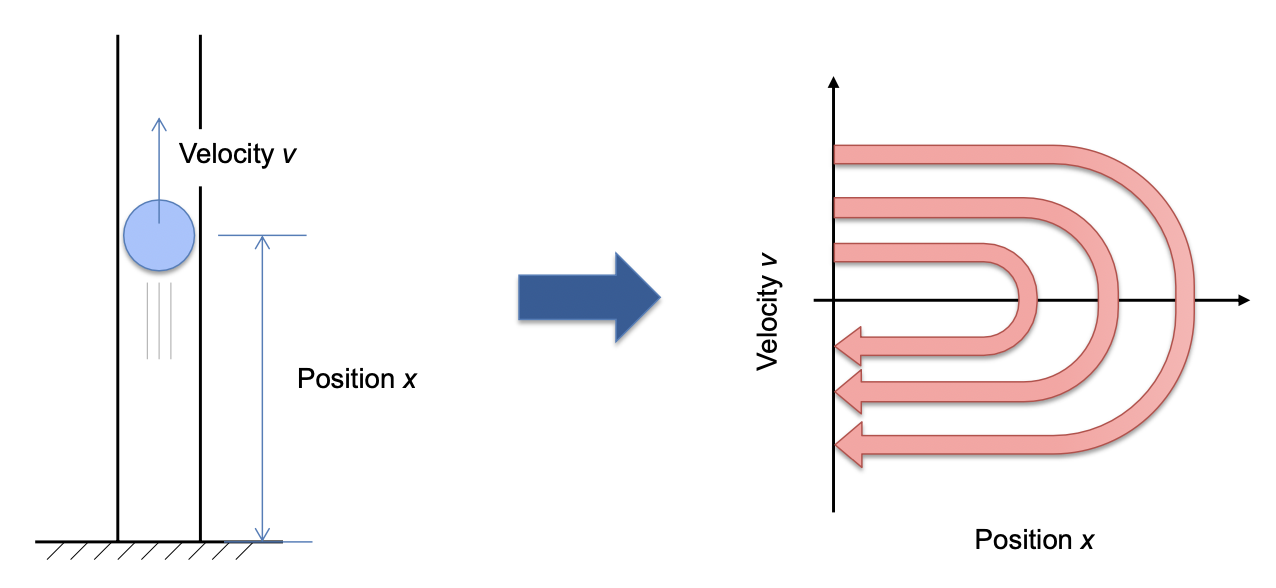
\includegraphics[width=0.6\textwidth]{phasespace.png}
        \caption{A ball thrown upward in a vertical tube (left) and a schematic illustration of
its phase space (right). The dynamic behavior of the ball can be visualized as a static
trajectory in the phase space (red arrows). (Source: H. Sayama, \emph{Introduction to the Modeling and Analysis of Complex Systems}, 2015, CC BY-NC-SA)}
    \end{figure}

\end{frame}

% Slide: Benefits of Drawing a Phase Space
\begin{frame}
    \frametitle{Benefits of Drawing a Phase Space}

    \textbf{Advantages of Phase Space:}
    \begin{itemize}
        \item A phase space diagram represents the dynamic behavior of a system as a \textbf{static trajectory}.
        \item This visualization provides intuitive, geometrical insights into the system's dynamics.
        \item Allows for easier interpretation compared to purely algebraic equations.
    \end{itemize}

\end{frame}

% Slide 1: Long-Term Behavior and Determinism in Phase Space
\begin{frame}
    \frametitle{What Can We Learn from Phase Space?}

    \textbf{Long-Term Behavior}
    \begin{itemize}
        \item In a deterministic dynamical system, the future state is uniquely determined by its current state.
        \item Phase space trajectories do not branch (only merge), ensuring that each initial state has a unique trajectory.
        \item By observing trajectories, we can determine if they:
            \begin{itemize}
                \item Diverge to infinity
                \item Converge to a point
                \item Remain confined within a region
            \end{itemize}
        \item \textbf{Attractors:} Points or regions where trajectories converge, representing stable long-term behaviors in complex systems.
    \end{itemize}
\end{frame}

% Slide 2: Basins of Attraction and Sensitivity to Initial Conditions
\begin{frame}
    \frametitle{Basins of Attraction and Initial Conditions}

    \textbf{Basins of Attraction}
    \begin{itemize}
        \item For each attractor, there exists a set of initial states that lead to it, called the \textbf{basin of attraction}.
        \item Multiple attractors in phase space allow us to divide it into regions, showing different possible outcomes.
    \end{itemize}

    \textbf{Sensitivity to Initial Conditions}
    \begin{itemize}
        \item A dominant region in phase space means that initial conditions have little impact on the system's fate.
        \item Multiple regions indicate \textbf{sensitivity} to initial conditions, where small changes can lead to different outcomes.
    \end{itemize}
\end{frame}


% Slide 1: Definition of Attractor
\begin{frame}
    \frametitle{Attractor}

	\begin{block}{Definition}
    \begin{itemize}
        \item An attractor \( A \) in a dynamical system is a set in the phase space.
        \item For a neighborhood of initial states \( x_0 \) around \( A \), the trajectory \( x(t) \) as \( t \to \infty \) tends toward \( A \).
    \end{itemize}
    
    \[
    \lim_{t \to \infty} d(x(t), A) = 0
    \]
    where \( d(x(t), A) \) is the distance between \( x(t) \) and \( A \).
\end{block}
\end{frame}

% Slide 2: Intuitive Explanation of Attractor
\begin{frame}
    \frametitle{Intuitive Explanation of Attractor}

    \begin{itemize}
        \item An attractor  \( A \) is a point or set of points in phase space that represents a stable state the system tends toward over time.
        \item Once the system is near the attractor, it will stay near or move closer to it as time progresses.
    \end{itemize}
    
    \bigskip
    Example: Imagine a pendulum swinging in air. Because of friction, it gradually loses energy and eventually stops at the lowest point. This bottom position is a \emph{stable attractor}, since the system tends toward it over time.
\end{frame}

% Slide 3: Definition of Basin of Attraction
\begin{frame}
    \frametitle{Basin of Attraction}

    \begin{block}{Definition}
    \begin{itemize}
        \item The \textbf{basin of attraction} for an attractor \( A \) is the set of all initial states \( x_0 \) that will ultimately move towards \( A \) over time.
    \end{itemize}

    Mathematically:
    \[
    B(A) = \{ x_0 \in \mathbb{R}^n : \lim_{t \to \infty} d(x(t), A) = 0 \}
    \]
    where \( d(x(t), A) \) is the distance between \( x(t) \) and \( A \).
\end{block}
\end{frame}

% Slide 4: Intuitive Explanation of Basin of Attraction
\begin{frame}
    \frametitle{Intuitive Explanation of Basin of Attraction}

    \begin{itemize}
        \item The basin of attraction is like a "zone of influence" around an attractor.
        \item Any starting point within this zone will lead the system to the attractor as time goes on.
    \end{itemize}
    
    \bigskip
    Example: For a ball in a bowl, the basin of attraction includes all points in the bowl, as no matter where you start the ball, it will eventually settle at the bottom (the attractor).
\end{frame}

% Slide 3: Stability of System States
\begin{frame}
    \frametitle{Stability of System States}

    \textbf{System Stability}
    \begin{itemize}
        \item Converging trajectories in phase space indicate \textbf{stable states}.
        \item Diverging trajectories indicate \textbf{unstable states}.
    \end{itemize}

    \bigskip

    Stability analysis is crucial for understanding, designing, and controlling real-world systems.

\end{frame}

\begin{frame}
	\frametitle{Reflection}
For each of the phase spaces shown below, identify the following:
\begin{itemize}
\item attractor(s)
\item basin of attraction for each attractor
\item stability of the system's state at several locations in the phase space
\end{itemize}

 \begin{figure}
        \centering
        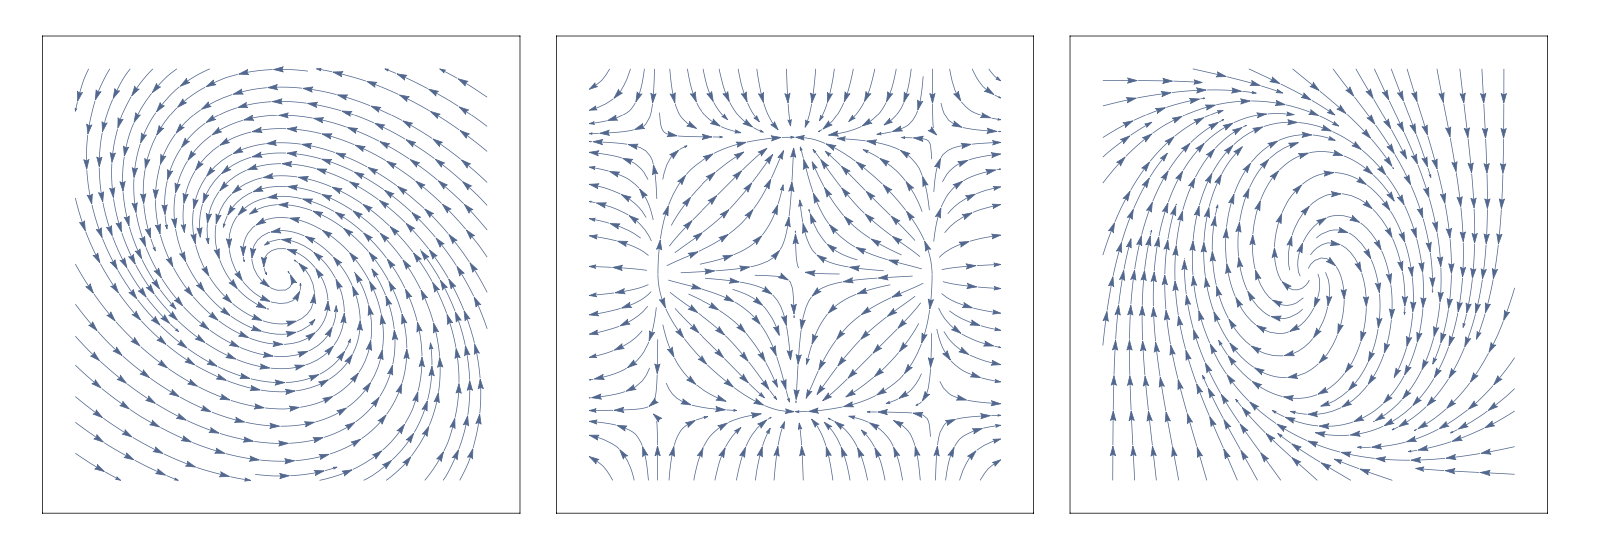
\includegraphics[width=0.6\textwidth]{attractor.png}
        \caption{Source: H. Sayama, \emph{Introduction to the Modeling and Analysis of Complex Systems}, 2015 (CC BY-NC-SA)}
    \end{figure}

\end{frame}

\section{Exercise at home}
\subsection{Market Competition}
% Slide 1: Exercise Frame - Market Competition
\begin{frame}
    \frametitle{Market Competition Between Products A and B}

    Consider a market with two equally good products, A and B, competing for market share.
    
    \bigskip
    
    There is a customer review website where users submit ratings. Although the average ratings are similar, customers can see the \textbf{total number of reviews}, influencing their choice due to popularity.

    \bigskip

    \textbf{Questions:}
    \begin{enumerate}
        \item What would the phase space of this system look like?
        \item Are there any attractors? Are there any basins of attraction?
        \item How does the system's fate depend on its initial state?
        \item If you were in charge of marketing product A, what would you do?
    \end{enumerate}
\end{frame}

% Slide 2: Hint for Phase Space
\begin{frame}
    \frametitle{Hint for Question 1: Phase Space}

    \textbf{Hint:}
    \begin{itemize}
        \item Consider the market share of each product as state variables.
        \item Think of a two-dimensional phase space where each axis represents the market share of products A and B.
        \item The sum of the two market shares should be constant (e.g., 100\% of the market), which could create a constraint in phase space.
    \end{itemize}
\end{frame}

% Slide 3: Hint for Attractors and Basins of Attraction
\begin{frame}
    \frametitle{Hint for Question 2: Attractors and Basins of Attraction}

    \textbf{Hint:}
    \begin{itemize}
        \item An attractor in this context could represent a stable market share distribution between the two products.
        \item Think about whether one product could end up dominating the market or if there could be a balance.
        \item The basin of attraction could indicate initial conditions (market share) that lead to one product becoming more popular.
    \end{itemize}
\end{frame}

% Slide 4: Hint for System?s Dependence on Initial State
\begin{frame}
    \frametitle{Hint for Question 3: System's Dependence on Initial State}

    \textbf{Hint:}
    \begin{itemize}
        \item Consider if a slight advantage in initial popularity could drive a product to dominate due to customer preference for the more popular choice.
        \item Think about how \emph{path dependency} might play a role in the evolution of the system.
    \end{itemize}
\end{frame}

% Slide 5: Hint for Marketing Strategy for Product A
\begin{frame}
    \frametitle{Hint for Question 4: Marketing Strategy for Product A}

    \textbf{Hint:}
    \begin{itemize}
        \item If popularity influences customer choice, what strategies could you implement to boost the perceived popularity of Product A?
        \item Consider incentivizing early adopters to submit reviews or focusing on visibility in initial stages.
    \end{itemize}
\end{frame}

% Slide 1: Solution - Phase Space
\begin{frame}
    \frametitle{Solution: Phase Space of Market Competition}

    \textbf{Phase Space:}
    \begin{itemize}
        \item The phase space can be represented with the market share of Product A on one axis and Product B on the other.
        \item Since the total market share is 100\%, this constrains the phase space to a line where:
        \[
        \text{Market Share of A} + \text{Market Share of B} = 100\%
        \]
        \item As a result, this phase space is one-dimensional, showing how the market share shifts between products.
    \end{itemize}
\end{frame}

% Slide 2: Solution - Attractors and Basins of Attraction
\begin{frame}
    \frametitle{Solution: Attractors and Basins of Attraction}

    \textbf{Attractors:}
    \begin{itemize}
        \item Potential attractors in this system are the points where one product fully dominates the market.
        \item These attractors represent stable states: either 100\% market share for Product A or for Product B.
    \end{itemize}

    \bigskip

    \textbf{Basins of Attraction:}
    \begin{itemize}
        \item Each attractor has a basin of attraction defined by the initial market share.
        \item If Product A starts with a higher initial market share, it is more likely to attract more customers, making it the basin of attraction.
        \item Similarly, a larger initial share for Product B makes it the basin for B's dominance.
    \end{itemize}
\end{frame}

% Slide 3: Solution - Dependence on Initial State
\begin{frame}
    \frametitle{Solution: Dependence on Initial State}

    \textbf{System's Fate and Initial State:}
    \begin{itemize}
        \item The system's outcome is highly sensitive to initial conditions due to customer preference for the more popular product.
        \item A small initial advantage in market share for one product can lead to that product ultimately dominating the market.
        \item This sensitivity illustrates \textbf{path dependency}, where early advantages strongly influence the final outcome.
    \end{itemize}
\end{frame}

% Slide 4: Solution - Marketing Strategy for Product A
\begin{frame}
    \frametitle{Solution: Marketing Strategy for Product A}

    \textbf{Suggested Strategy for Product A:}
    \begin{itemize}
        \item \textbf{Boost initial popularity:} Increase initial customer engagement and reviews to create an early advantage.
        \item \textbf{Incentivize reviews:} Encourage existing customers to submit positive reviews to boost visibility and perceived popularity.
        \item \textbf{Increase visibility:} Promote Product A aggressively at launch to attract early adopters, enhancing its perceived popularity.
    \end{itemize}

    By focusing on these strategies, Product A can gain a competitive edge, which may lead to capturing a larger market share in the long run.
\end{frame}

\subsection{Predator-Prey System}

% Slide 1: Introduction to the Lotka-Volterra System
\begin{frame}
    \frametitle{Exercise: The Lotka-Volterra System}

    The \textbf{Lotka-Volterra equations} describe the dynamics between two species: a \textbf{predator} and its \textbf{prey}. This system of differential equations is given by:

    \[
    \frac{dx}{dt} = \alpha x - \beta x y
    \]
    \[
    \frac{dy}{dt} = \delta x y - \gamma y
    \]

    where:
    \begin{itemize}
        \item \( x \) represents the prey population.
        \item \( y \) represents the predator population.
        \item \( \alpha, \beta, \delta, \gamma \) are positive constants representing interaction rates.
    \end{itemize}
\end{frame}

% Slide 2: Questions for Analysis
\begin{frame}
    \frametitle{Questions for Analysis}

    \begin{enumerate}
        \item Draw the \textbf{state space} (populations of prey and predator over time) for the Lotka-Volterra system.
        \item Draw the \textbf{phase space} (predator population versus prey population).
        \item Are there any \textbf{attractors} in this system? If so, where?
        \item Describe the type of dynamics you observe (e.g., cycles, convergence, or divergence).
        \item What happens to the populations if we increase the interaction rate \( \beta \) (impact of predators on prey)?
    \end{enumerate}
\end{frame}

\begin{frame}
    \frametitle{State and Phase Space of Lotka-Volterra System}

    \begin{columns}
        \column{0.5\textwidth}
        \textbf{State Space Plot:}
        \begin{itemize}
            \item Shows populations of prey (\( x \)) and predator (\( y \)) over time.
        \end{itemize}
        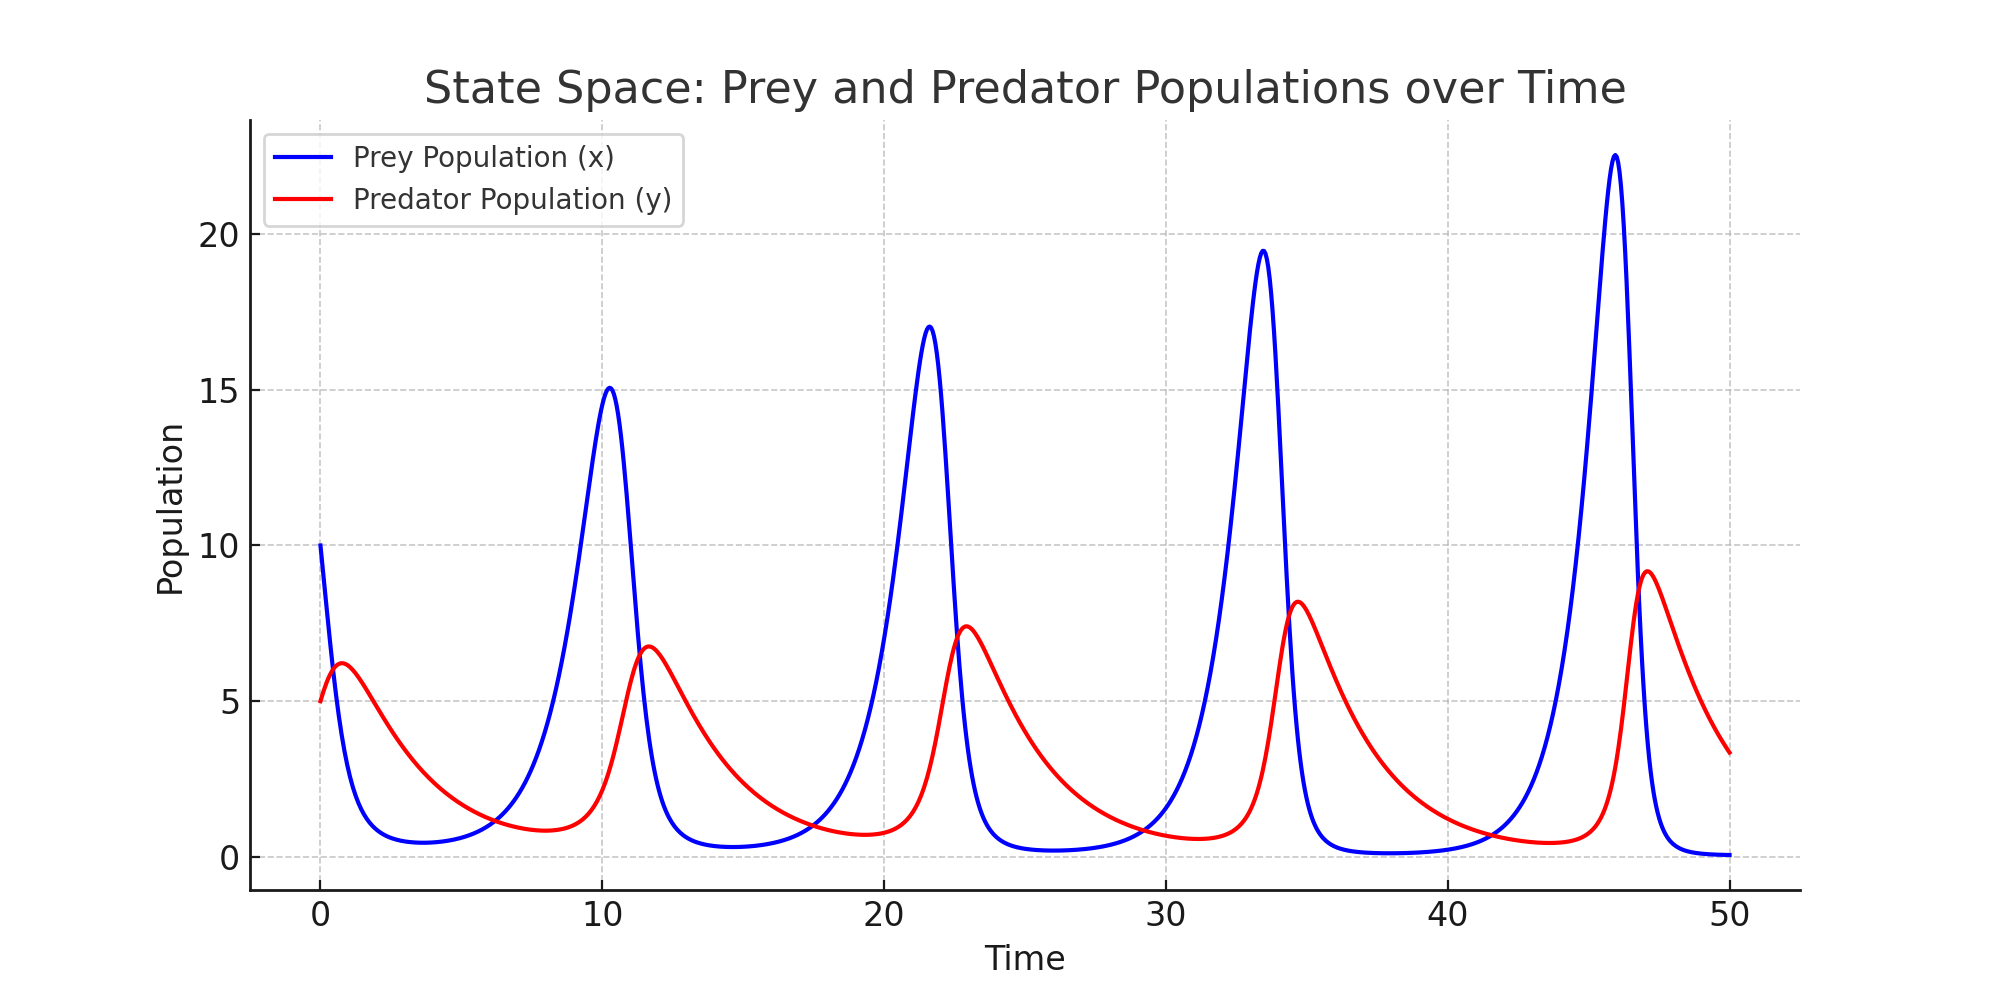
\includegraphics[width=\textwidth]{lotka_volterra_state_space.png}

        \column{0.5\textwidth}
        \textbf{Phase Space Plot:}
        \begin{itemize}
            \item Shows the relationship between predator and prey populations.
        \end{itemize}
        \centering
        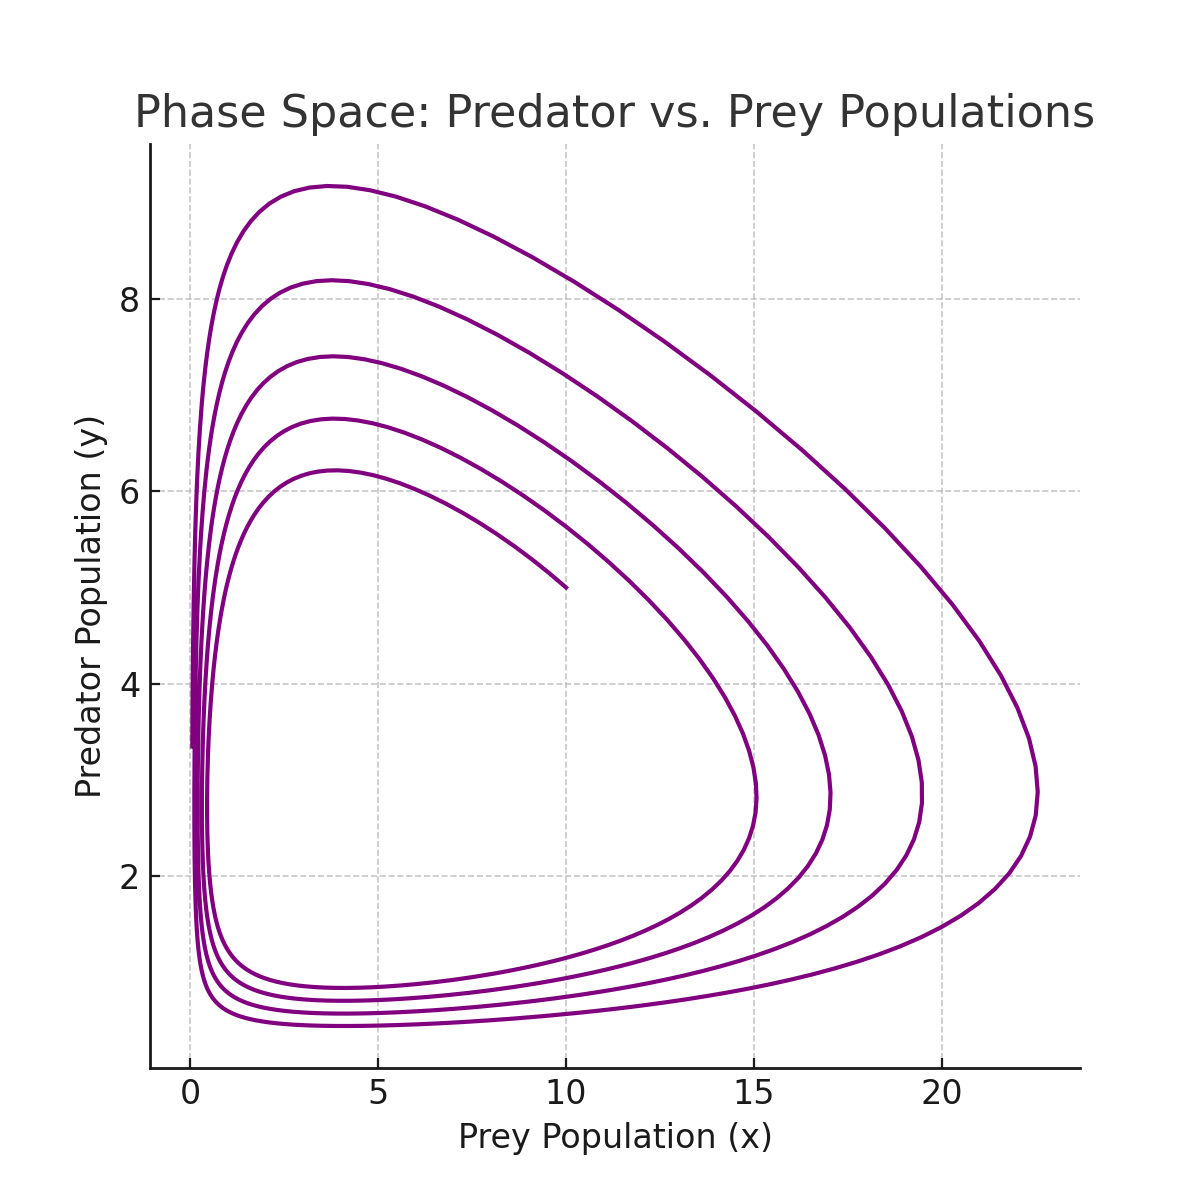
\includegraphics[width=0.5\textwidth]{lotka_volterra_phase_space.png}
    \end{columns}

\end{frame}

% Slide 5: Hints for Analysis
\begin{frame}
    \frametitle{Hints for Analysis}

    \begin{itemize}
        \item For \textbf{state space}, plot prey and predator populations as functions of time.
        \item For \textbf{phase space}, consider how predator and prey populations interact with each other, often forming closed cycles.
        \item Check for any points where the populations remain constant or stabilize over time?these may be attractors.
        \item Increasing \( \beta \) intensifies predation. Consider the impact on prey and predator populations over time.
    \end{itemize}
\end{frame}

\end{document}